% This is LLNCS.DEM the demonstration file of
% the LaTeX macro package from Springer-Verlag
% for Lecture Notes in Computer Science,
% version 2.4 for LaTeX2e as of 16. April 2010
%
\documentclass{llncs}
%
\usepackage{makeidx}  % allows for indexgeneration
%
\usepackage{graphicx}

\usepackage{mathtools}
\DeclarePairedDelimiter{\norm}{\lVert}{\rVert}
\DeclareMathOperator*{\argmin}{argmin}

\setcounter{secnumdepth}{4} % seting level of numbering (default for "report" is 3).

% define a newline after subsubsection like subsection
\makeatletter
\renewcommand\subsubsection{\@startsection{subsubsection}{3}{\z@}%
	{-18\p@ \@plus -4\p@ \@minus -4\p@}%
	{4\p@ \@plus 2\p@ \@minus 2\p@}%
	{\normalfont\normalsize\bfseries\boldmath
		\rightskip=\z@ \@plus 8em\pretolerance=10000 }}
\makeatother


\begin{document}
%
\frontmatter          % for the preliminaries
%
\pagestyle{headings}  % switches on printing of running heads


%

%
\mainmatter              % start of the contributions
%
\title{Yelp Recommendation System Based on Collaborative Filtering}
%
\titlerunning{Yelp Recommendation System Based on Collaborative Filtering}  % abbreviated title (for running head)
%                                     also used for the TOC unless
%                                     \toctitle is used
%
\author{Sainan He, Jiaoyang Fu, Yameng Li}
%
\authorrunning{Ivar Ekeland et al.} % abbreviated author list (for running head)
%
%%%% list of authors for the TOC (use if author list has to be modified)
\tocauthor{Sainan He, Jiaoyang Fu, Yameng Li}
%
\institute{Electrical and Computer Engineering, University of Waterloo, Canada,\\
\email{{s66he, j45fu, y949li}@uwaterloo.cau}
}

\maketitle              % typeset the title of the contribution

\begin{abstract}

Based on Yelp Data Challenge dataset, we aim to develop a predictive personalized recommendation system on user’s review star rating for restaurants, applying collaborative filtering algorithms. In particular, we implement and compare the performances of four algorithms including baseline, User-based and Item-based collaborative filtering and Singular Value Decomposition (SVD). We evaluate our results by comparing our predicted rating to the actual rating using Root Mean Squared Error(RMSE) and Mean Absolute Error(MAE) metrics.

\keywords{Recommendation System, Collaborative filtering, Singular Value Decomposition (SVD), Yelp Data Challenge}
\end{abstract}

\section{Introduction}
With rapid development of advanced technology, people nowadays can achieve the things that they desired faster and more effectively than ever by recommendations. The recommendation system is now widely used in various of applications, such as movies, books, musics and web pages. Despite of the vast amount of application, the requirements for accurate, personalized and convenient services are increasing. 

More than ever before, people's decisions of where to visit or what to eat are subject to other people's opinions. Yelp is a popular crowd-sourced local business reviews and social networking platform making it become an important reference for making consumer decision. For each individual business, users can submit a review on their products or services using a one to five star rating system as well as text comments.

Collaborative filtering, a method of making predictions based on a large dataset is used by many recommendation system like Yelp, Amazon, and Netflix. It automatically predict about the interests of a user by collecting preference or tastes information from other users. Furthermore, there are numerous collaborative filtering methods, such as user-based CF, item-based CF, and matrix decomposition. 

Through this project we utilized Yelp's data to make personalized business recommendations for Yelp users by predicting the rating that a given user would give to a specific business.

In section 2 we introduce the related work about recommendation systems including the methods they used and their related results. Contents from section 3 to the final part are about our own work. We begin by describing the dataset used to predict ratings. We then elaborate on the different models used to predict the rating that a user would assign to a business. This is followed by a description of the evaluation metric and implementation. Finally, we conclude with our results, discussion and talk briefly about future direction.

\section{Literature Review}
There are generally three types of recommendation systems: content-based filtering, collaborative filtering and hybrid approaches. Content-based recommendation systems work with users' profile and items' characteristics. The feature used to build profiles are often a set of keywords. For example, a music recommendation system\cite{MJ} implemented with content-based filtering, each song is assigned an attribute manually. If a user’s profile shows interests in songs with particular attributes, similar songs will be recommended to the user. The limitations of these systems is that it always recommends similar items to user that he has already purchased and it’s difficult to recommend items for new users. 

Collaborative filtering try to predict the utility of items for a particular user based on the items previously rated by other users with similar tastes and preferences. In\cite{Bruno} the author builds a recommendation system for a retail store using three kinds of collaborative filtering algorithms - memory based approach, matrix factorization and bigram matrix method. Collaborative filtering also has limitations that it is difficult to recommend items for new users, to recommend items which have not been rated before, and to recommend when rating information is insufficient. 

Hybrid approach combines multiple techniques to overcome the limitations of individual systems. A restaurant recommendation system for yelp user\cite{Sumedh} adopts hybrid approach by extracting collaborative and content-based features to identify customer and restaurant profiles. A hybrid cascade of K-nearest neighbor clustering, weighted bi-partite graph projection, and several other learning algorithms are proposed. 

\section{Data}
We collect our data from Yelp recommendation Kaggle competition\cite{yelp},This dataset contains 11,537 businesses, 8282 check-in sets, 43873 users, and 229907 reviews. Each user has a unique user id as well as business. We target ``Restaurant'' in the city of ``Phoenix'' as it is more reasonable to recommend restaurants for users in the same city and Phoenix has the most amount of review records among all the cities.
\subsection{ Data Processing}
The original data file is in json format. We firstly parse the raw data of information from users, businesses and reviews, respectively and merge them into one dataframe. Then we extract the records with features of “Restaurants” and “Phoenix” for further analysis. After this approach, we have 17145 users, 1454 business and 52749 reviews.

Because many users only review a few restaurants, our dataset yields a sparsity of 99.79\% which can be visualized from figure 1. To solve this problem, we create a smaller dataset which only consider  restaurants reviewed by more than 50 users.
%

\begin{figure}
	\begin{minipage}[t]{0.5\textwidth}
		\centering
		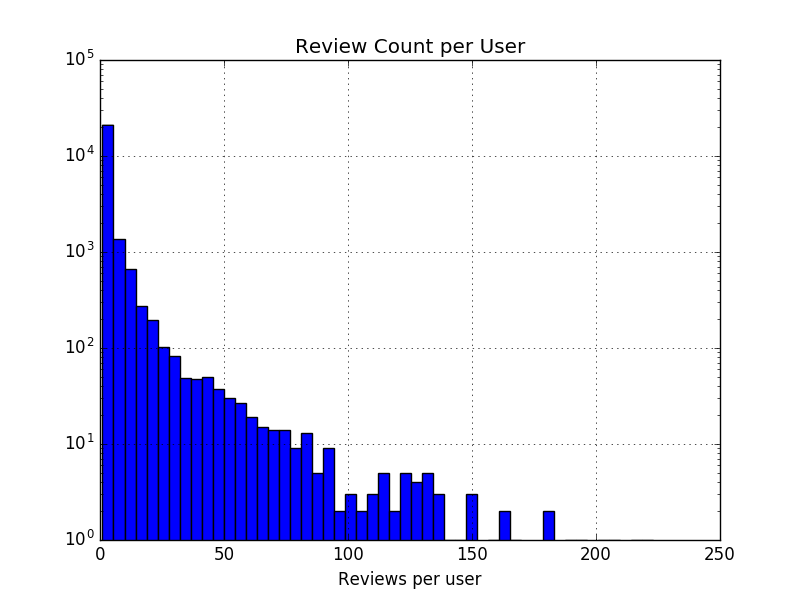
\includegraphics[width=2.2in]{fig1.png}
		\caption{User review count}
		\label{fig:side:a}
	\end{minipage}%
	\begin{minipage}[t]{0.5\textwidth}
		\centering
		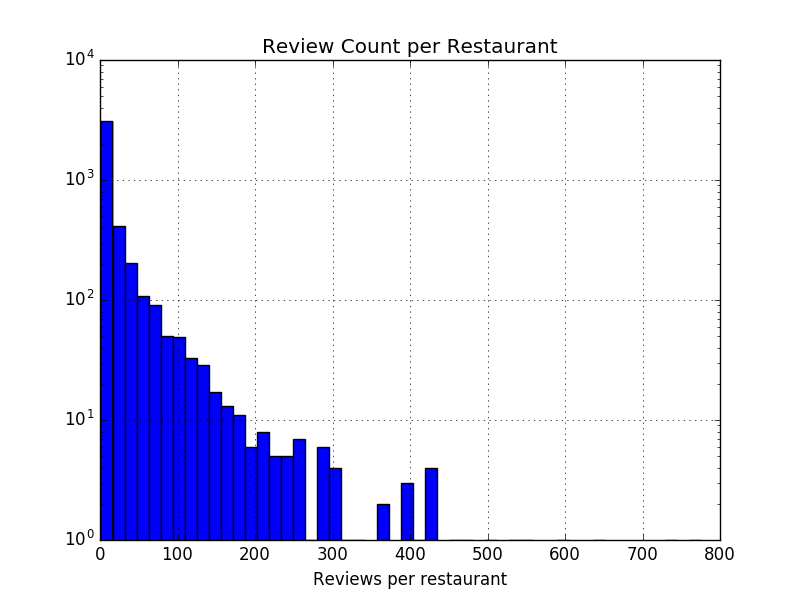
\includegraphics[width=2.2in]{fig2.png}
		\caption{Restaurants review count}
		\label{fig:side:b}
	\end{minipage}
\end{figure}

\subsection{Training and Testing sets}
%
In order to evaluate the performance of our recommendation system, we divided our data into training and testing datasets. We extract a list of all restaurants each user has rated, take 80\% of this list as training set and 20\% as test set. 

\section{Methods}
\subsection{Baseline}
Our baseline model is similar to the model implemented by\cite{Yehuda} which is a mean predictor and accounts for the user and item effects. 
\begin{equation}
\ b_{ur} = \mu + b_u + b_r \ .
\end{equation}

Here $\mu$ is the mean rating of reviews of all business by all users. The parameter $b_{ur}$ indicates the difference between the average rating of user $u$ and $\mu$. The parameter bi indicates the difference between the average rating of business $i$ and $\mu$. This will normalize the widely noticed tendency of some user giving higher rating than others and some restaurants getting higher ratings than others.


\subsection{User-User Collaborative Filtering}
\textit{User-user collaborative filtering}, also know as \textit{k-NN collaborative},was the first of the automated CF methods. It find other users whose past rating behavior is similar to that of current user and
use their ratings on that item to predict what the current user will like. To predict Mary's preference for an item she has not rated, user-User CF looks for other users who have high agreement with Mary on the items they have both rated.These users’ ratings for the item in question are then weighted by their level of agreement with Mary’s ratings to predict Mary's rating on that item. 

\subsubsection{Computing Predictions}
To compute predictions or recommendations for a user u, user-user CF firstly needs to determine the number N of neighbors will be used to generate the result. Then computing the weighted average of the chosen neighboring users' rating i by using similarity as weights. The formula is given as below:

\begin{equation}
p_{u,i} ={\bar r_{u}}  + \frac
{\sum\nolimits_{u' \in N} s(u,u')(r_{u',i} - {\bar r_{u'}})} 
{\sum\nolimits_{u' \in N} |s(u,u')|}
\end{equation}

In order to eliminate the differences in users's use of the rating scale, subtracting the user's mean rating ${\bar r_{u'}}$ to compensate is necessary.   The parameter $p_{u,i}$ is predicated rating on item i for user $u$.  ${\bar r_{u'}}$ is average rating on all items rated by user $u$.The parameter $r_{u',i}$ indicates the rating of user $u'$ on item i.$s(u,u')$ is similarity between user u and $u'$. N is the number of neighbors chosen for user $u$.  



\subsubsection{Measure of Similarity}
An critical parameter used to calculate predications is similarity function. The most common and typically measurement are the cosine similarity and Pearson similarity. 

In Cosine Similarity model, users are represented as $|\textit{I}|$-dimensional vectors of rating on $|\textit{I}|$ items. Similarity is measured by the cosine distance between two rating vectors. The formula is given below indicating how to calculate the Cosine Similarity between user $u$ and $v$. 
\begin{equation}
s(u,v) = \frac{r_{u}\cdot r_{v}}{\norm {r_{u}}_{2} \norm {r_{v}}_{2}}=\frac{\sum\nolimits_{i} r_{u,i}r_{v,i}}{\sqrt{\sum\nolimits_{i} {r^{2}_{u,i}}} \sqrt{\sum\nolimits_{i} {r^{2}_{v,i}}}} 
\end{equation}

Unknown ratings are considered to be 0. $r_{u}$ is rating vector of user $u$. $\norm {r_{u}}_{2}$ is the Euclidean norm of rating vector $r_{u}$.

Unlike cosine similarity, the Pearson correlation is a measure of how well two sets of data fit on a straight line. It is slightly more sophisticated way to determine the similarity between users. A Pearson Correlation Coefficient of 1 indicates that the two users are perfectly correlated but in this case, a score of -1 means that the they are not correlated.

In our Pearson Correlation model, it computes the statistical correlation between two user's common ratings to determine their similarity. The formula is given below indicating how to calculate the Pearson Similarity between user $u$ and $v$. 

\begin{equation}
	s(u,v) =\frac{{\sum\nolimits_{i \in {I_{u} \cap I_{v}}}(r_{u,i}-\bar{r}_{u})(r_{v,i}-\bar{r}_{v})}}{ \sqrt{{\sum\nolimits_{i \in {I_{u} \cap I_{v}}}(r_{u,i}-\bar{r}_{u})^2}} \sqrt{{\sum\nolimits_{i \in {I_{u} \cap I_{v}}}(r_{v,i}-\bar{r}_{v})^2}}}
\end{equation}

The parameter $I_{u}$ is a set of items rated by user $u$. Parameter ${\bar r_{u}}$ is average rating on all items rated by user $u$.The parameter $r_{u,i}$ indicates the rating of user $u$ on item i.

\subsection{Item-Item Collaborative Filtering}
\textit{Item-Item Collaborative Filtering} is similar to User-User CF, it uses similarity between the rating patterns of items. If two items tend to have the same users like and dislike them,then they are similar and users are expected to have similar preferences for similar items.

To generate predictions or recommendations for user $u$ on item $i$, item-item CF firstly determine a set S of items most similar to $i$. Then we extracted k nearest neighbors of item i computing the weighted average of the user's rating on item $j$ from set S. The formula is given as below:

\begin{equation}
p_{u,i} =\frac
{\sum\nolimits_{j \in S} s(i,j)r_{u,j}} 
{\sum\nolimits_{j \in S} |s(i,j)|}
\end{equation}

The parameter $p_{u,i}$ is predicated rating on item i for user $u$. $S$ is a set of items most similar to item $i$. $s(i,j)$ is the similarity between item $i$ and $j$. $r_{u,j}$ is the rating of user $u$ on item $i$.

For item-item CF, we choose the Peason correlation to measure similarities. 


\subsection{Singular Value Decomposition}
Singular Value Decomposition(SVD) is a latent factor method which popularly applied in Netflix Prize competition. A matrix can be approximated with SVD by multiplying two generated feature matrices $P$ and $Q$ with rank $k$ \cite{Naomi}.
\begin{equation}
\hat{R_{ij}} = P_iQ_{j}^{T}
\end{equation}
In this paper, the matrix $R$ is a ratings matrix with rows representing all the users, and columns representing businesses. For example $R_{ij}$ represents the rating from user $i$ to restaurant $j$. Then, minimizing the squared differences between the rating matrix $R$ and the SVD approximated matrix $\hat{R}$. Thus, projecting user and restaurants rating matrix into two lower dimension feature matrices $P$ as user feature matrix and $Q$ as restaurant matrix. In order to improve the SVD prediction accuracy, subtract the global average rating, $\mu$.

\begin{equation}
\hat{R_{ij}} = P_iQ_{j}^{T} + \mu
\end{equation}

\begin{equation}
\argmin_{P,Q}\sum_{(i,j)\in{R}}{(R_{ij} - \mu - P_iQ_{j}^{T})}^2
\end{equation}

We also add a regularization to avoid overfitting to our training set.

\begin{equation}
\argmin_{P,Q}\sum_{(i,j)\in{R}}{(R_{ij} - \mu - P_iQ_{j}^{T})}^2 + \lambda({\left\|P_i\right\|}^2 + {\left\|Q_j\right\|}^2 )
\end{equation}

In order to find optimum matrices for $P$ and $Q$, we implement the alternating least squares method as described by Cichocki and Zhou\cite{Andrzej},\cite{Yunhong}.

After obtaining the predicted rating by matrices $P$ and $Q$ via SVD, add the global mean back to each predicted rating. We take $k$ as 20 and $\lambda$ as 0.01.

\section{Experiments and Results}
%
\subsection{Evaluation Metrics}
Our goal is to predict the rating a user would give to a restaurant. We predict the rating that user has not rated in the training dataset, but the true rating is stored in the test dataset. We use the root-mean-square error and mean-absolute error for evaluation.
\begin{equation}
\ RMSE = \sqrt{\frac{\sum{\left(r'_{u,i} - r_{u,i}\right)}^2}{N}}
\end{equation}
\begin{equation}
\ MAE = \sqrt{\frac{\sum{\left|r'_{u,i} - r_{u,i}\right|}}{N}}
\end{equation}

Here $r'_{u,i}$ is the predicted rating from user $u$ on item $i$ and $r_{u,i}$ is the true rating; $N$ is the size of test dataset. 
\subsection{Implementation}
\subsubsection{Program Structure}
Our work was implemented by Python. We have seven python files in total. They are main, loadData, Baseline, User-based CF, Item-based CF, SVD and Evaluation. The main program is the controller of the whole recommendation system. At first, it invoked the loadData file for data parsing. Then it invoked Baseline, User-based CF, Item-based CF and SVD predicting ratings using these four algorithms. Each time the predicted rating and true rating were stored together and the Evaluation program will calculate the RMSE and MAE errors for the predictions. 
\subsubsection{Data Structure}
We used Pandas for data processing which is an open source, data analysis library. The original json files were loaded into three dataframe storing information of users, business and reviews respectively. We joined the business and reviews dataframes based on business id and then joined with the users dataframe on user id. After parsing the raw data, we used the key ``Category'' and ``City'' to extract records of ``Restaurants'' and ``Phoenix''. As to reboost sparsity problem, we computed the count of reviews grouped by restaurant id and filtered the restaurants getting rid of the restaurants which had fewer than 50 reviews. 

After re-organizing the data, we used dictionary data structure to build the user-item matrix. For each records in the joined dataframe, we extract user as the key, the value of each key is a nested dictionary with business id as key and review rating as value, e.g. $\{user\_id: \{restaurant\_id: rating\}\}$. Meanwhile, we also built another item-user matrix which can be indexed by restaurant id, e.g. $\{restaurant\_id: \{user\_id: rating\}\}$.

For dividing data into training and testing data, we only consider users with more than 30 reviews. That is for each key in the user-indexed dictionary, if the length of the value set is greater than 30, we took 20\% of the entry out of the set and stored them into the test dictionary. The remaining 80\% became the training data. 

After this approach, we have 281 restaurants, 13820 users in training set and 91 users in test set.
\subsection{Baseline}
The joined dataframe was used to calculate overall average ratings $\mu$ that all users reviewed on all restaurants, average ratings $b_u$ of every users grouped by user id and average ratings $b_r$ of every restaurants grouped by restaurant id. These values were applied in equation(1) for the baseline prediction.

The performance of our baseline predictor is $RMSE = 0.9014 $, $MAE = 0.8397$.

\subsection{User-User CF and Item-Item CF}
By using the preprocessed training data and testing data, joined dataframe, prediction formula and similarity formula, we did four experiments to see the performance of each method under given conditions.   

\subsubsection{User-based CF with Cosine Similarity on Whole Data}
In this experiment, we used the resubstitution method which trained on all data and test on the same data set. Cosine similarity was used to measure similarities. 

\begin{figure}
	\begin{minipage}[t]{0.5\textwidth}
		\centering
		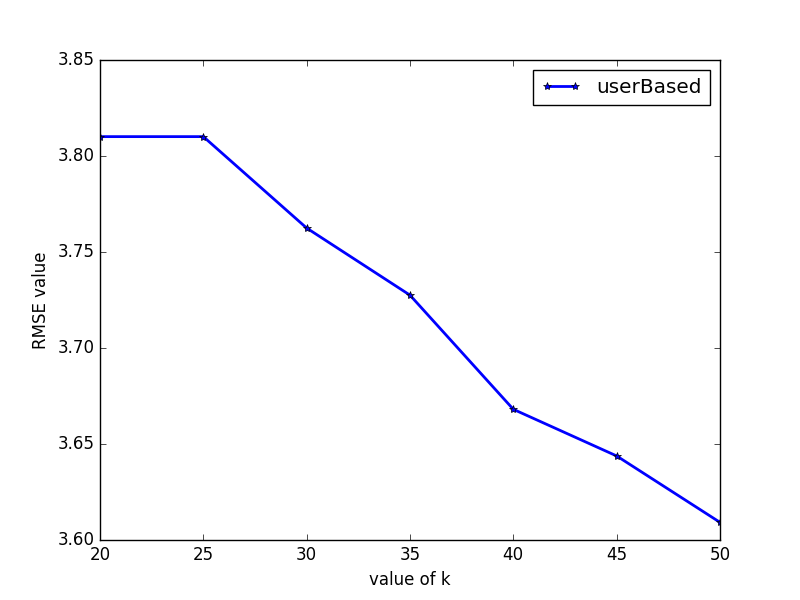
\includegraphics[width=2.2in]{RMSE1.png}
		\caption{Used-based RMSE}
		\label{fig:side:a}
	\end{minipage}%
	\begin{minipage}[t]{0.5\textwidth}
		\centering
		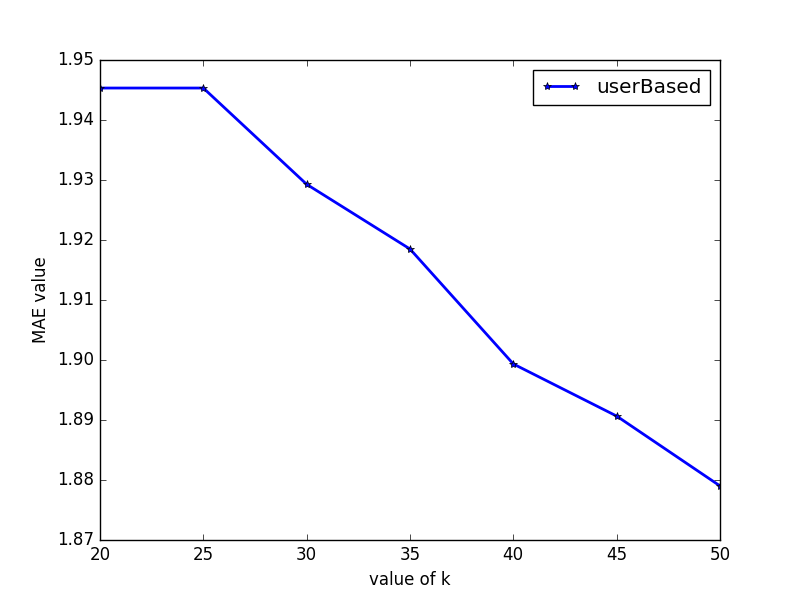
\includegraphics[width=2.2in]{MAE1.png}
		\caption{Used-based MAE}
		\label{fig:side:b}
	\end{minipage}
\end{figure}

K is the number of nearest neighbors chosen for each user when calculating the predicated ratings. we can see from figure 3 and figure 4 that both RMSE(greater than 3.8) and MAE value (about 1.95) are very high when k is 20. But with the increasing of k, both RMSE and MAE decrease quickly. This is because when more meaningful similar users are taking into consideration when calculating  ratings, the accuracy thus is improved. 

\subsubsection{User-based CF with Cosine Similarity on Divided Data}
In this experiment, we used holdout method which train on 80\% data and predicated ratings for users in the extracted 20\% testing data. Also cosine similarity was used to measure similarity. We can see from figure 5 and figure 6 that when k is 20,both RMSE and MAE reach their lowest value respectively.when k is lower than 20 or larger than 20, both RMSE and MAE increases. This is because if too many users with low similarity to current user are considered, the accuracy is negatively affected. Also, if not enough users with high similarity to current user are chosen, the accuracy cannot achieve the best. 

\begin{figure}
	\begin{minipage}[t]{0.5\textwidth}
		\centering
		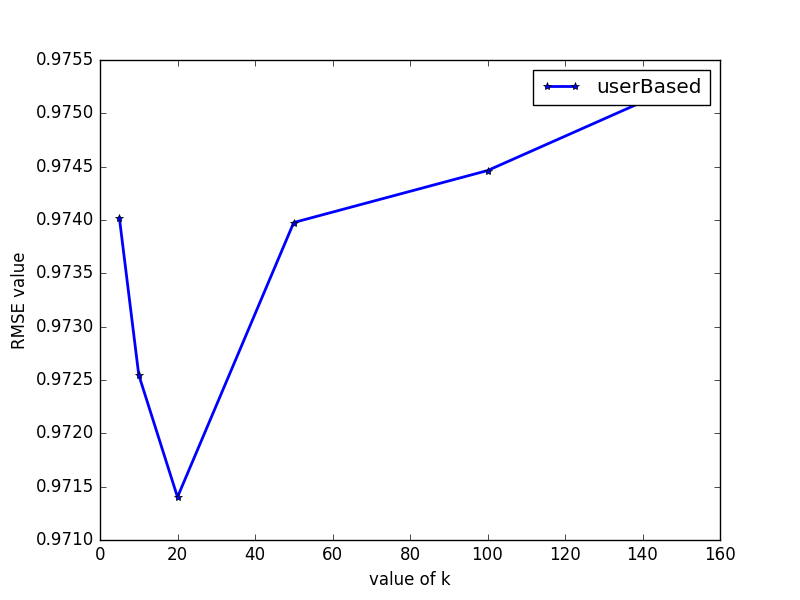
\includegraphics[width=2.2in]{RMSE2.png}
		\caption{Used-based RMSE}
		\label{fig:side:a}
	\end{minipage}%
	\begin{minipage}[t]{0.5\textwidth}
		\centering
		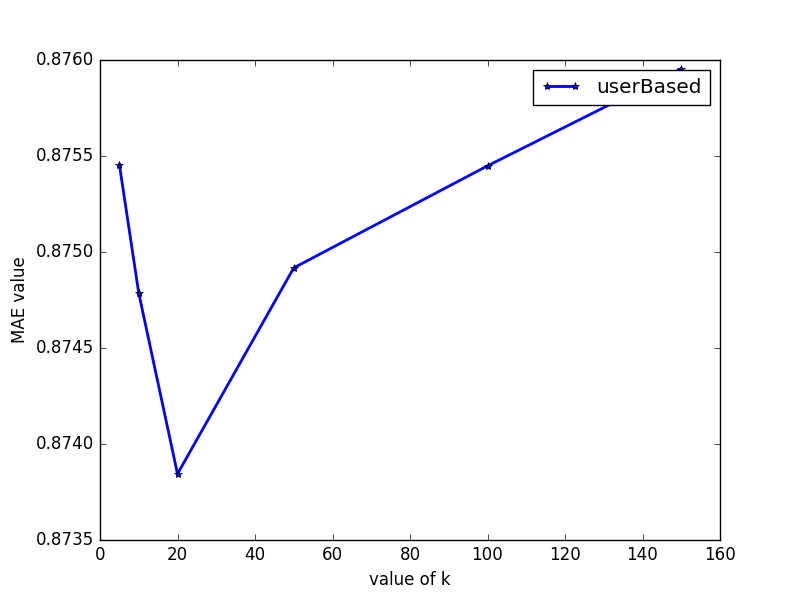
\includegraphics[width=2.2in]{MAE2.png}
		\caption{Used-based MAE}
		\label{fig:side:b}
	\end{minipage}
\end{figure}
 

\subsubsection{User-based CF with Pearson Similarity on Divided Data}
We used Pearson correlation instead of cosine distance to measure similarities. Figure 7 and figure 8 shows that when k is in the range of 5 to 50, both RMSE and MAE value decrease dramatically with the increasing of k. After 50, with the increasing of k,both both RMSE and MAE value decrease slowly. This is because the similarity whose ranking behind  50 has lower effect on the predicted ratings.

\begin{figure}
	\begin{minipage}[t]{0.5\textwidth}
		\centering
		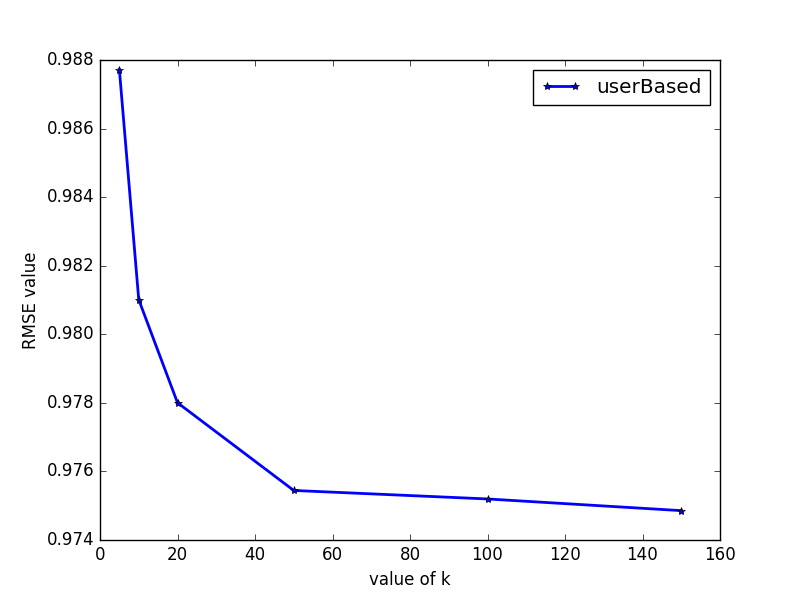
\includegraphics[width=2.2in]{RMSE3.png}
		\caption{Used-based RMSE}
		\label{fig:side:a}
	\end{minipage}%
	\begin{minipage}[t]{0.5\textwidth}
		\centering
		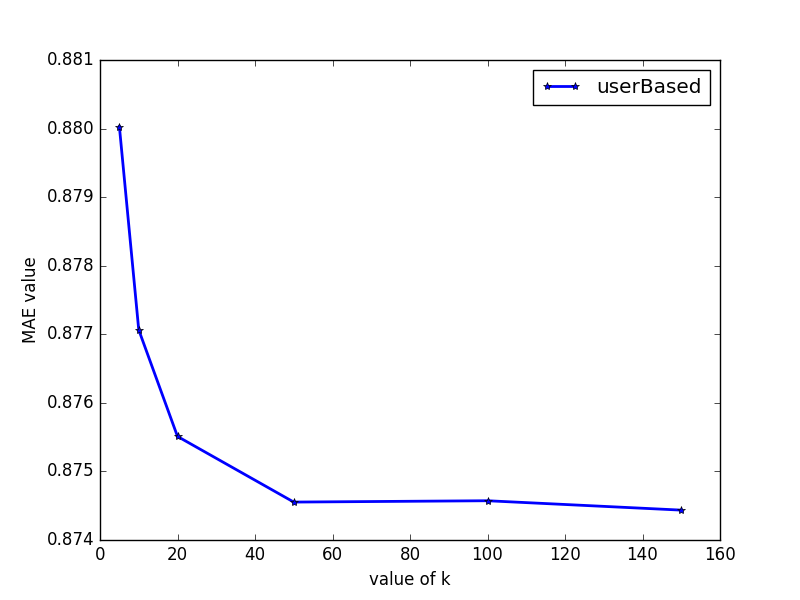
\includegraphics[width=2.2in]{MAE3.png}
		\caption{Used-based MAE}
		\label{fig:side:b}
	\end{minipage}
\end{figure}


\subsubsection{Item-based CF with Pearson Similarity on Divided Data}
In this experiment, we applied the item-based CF to find the the k nearest neighbours of each restaurant. The similarity between items were measured by pearson correlation.  

\begin{figure}
	\centering
	\begin{minipage}[t]{0.5\textwidth}	
		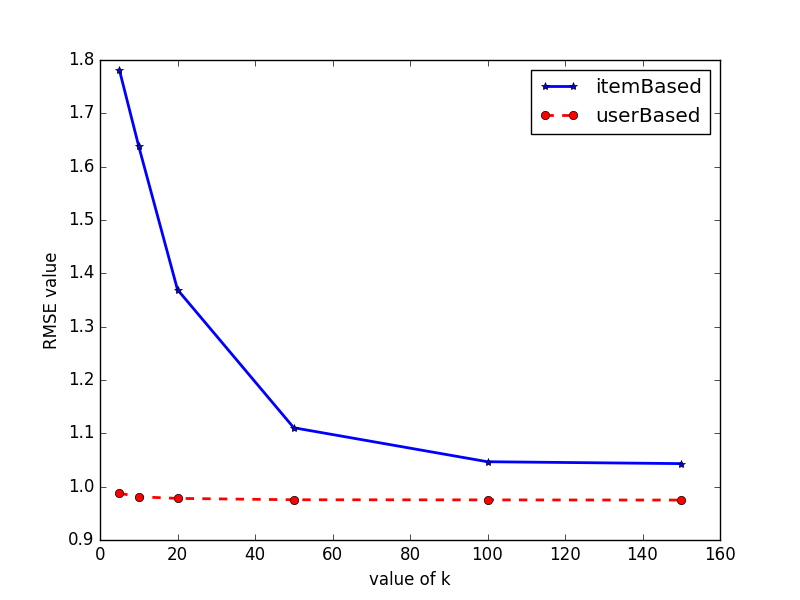
\includegraphics[width=2.2in]{twoPearsonMethods.png}
		\caption{Used-based RMSE}
		\label{fig:side:a}
	\end{minipage}
\end{figure}

We changed the value of k and compared the result of item-based prediction with user-based prediction, we can see from figure 9 that under the same given conditions, user-based prediction surpasses item-based prediction. This is because pearson correlation is more suitable for calculating similarity for user based prediction. 

\subsection{SVD}
According to the training set, we use SVD method to generate two matrices $P$ and $Q$ which represent User matrix and Restaurant matrix respectively. We choose the decreased dimension $K-factors = 20$, and regularization $\lambda = 0.01$. Then we use these two matrices $P$ and $Q$ to form a predicted matrix. Then we use the testing set to measure how well SVD works by RMSE and MAE method.

When applying SVD method to the yelp data, at first we did not minus the global average rating value, the RMSE result is 1.0568, which indicates the method works not that well comparing to other methods. To improve SVD, we subtracted the global average rating value first to generate the metrics $P$ and $Q$, after generating the predicted matrix, adding the global average rating value to each element. The RMSE result improves to  0.9175. Analyzing this phenomenon, it may note that in the origin matrix of rating between users and restaurants contains too many latent value. Thus, if we do not use global average value to control the latent value, it will badly influence the SVD performance measured by RMSE.

\subsection{Comparison}
Table 1 shows the RMSE and MAE of each applied algorithms.
\begin{table}
	\caption{Performance of four algorithms for recommendation system}
	\begin{center}
		\begin{tabular}{ccc}
			\hline
				\rule{0pt}{12pt}Method  & \rule{0pt}{12pt}RMSE   &\rule{0pt}{12pt} MAE\\
			\hline\rule{0pt}{12pt}
			Baseline    &   0.9014 & \ 	0.8397 \\
			User-based  &   0.9754 & \ 	0.8745\\
			Item-based  &   1.1106 & \      0.9217\\
			SVD         &   0.9175 & \      0.8403\\
			\hline
		\end{tabular}
	\end{center}
\end{table}

\section{Discussion and Future Work}
From table 1 we can see that the baseline which is a mean predictor yields the best result. It is not surprising that collaborative filtering does not work very well with the yelp dataset. As we cited in the data section, the number of users who have reviewed enough restaurants for calculating similarity scores with other users is quite low. Collaborative filtering usually works not well when data are sparse, and has cold start problem for new users and items.

For the SVD, several parameters can influence the performance, such as decreased dimension, and regularization. As we know, for a fixed number of samples the best number of features would be some intermediate value rather than the smallest or biggest which is the peak phenomenon. For our project, we can adjust the regularization and learning rate parameters, changing the number of features under each pairwise, finally choose the best parameters with lowest error. This may help to improve SVD accuracy.
 
 In the future work, we would consider the classification of restaurants and apply our approaches based on the classification. Another method is to analyze the review text which is provided in the review json file and use this information to create comprehensive user and restaurant profiles. Also, we would explore further hybrid approaches and evaluate their performances.

%
% ---- Bibliography ----
%
\begin{thebibliography}{5}
%
\bibitem {MJ}
MJ Pazzani, D Billsus.:
Content-based Recommendation Systems. In The adaptive web, pp. 325–341. Springer (1981) 

\bibitem {Bruno}
Bruno Pradel, Savaneary Sean, Julien Delporte.: 
A Case Study in a Recommender System Based on Purchase Data. Proceedings of the 17th ACM SIGKDD international conference on Knowledge discovery and data mining, pp. 377-385 (2011)

\bibitem {Sumedh}
Sumedh Sawant, Gina Pai.:
Yelp Food Recommendation System

\bibitem {yelp}
https://www.kaggle.com/c/yelp-recsys-2013

\bibitem {Yehuda}
Yehuda Koren.: 
Factorization meets the neighborhood: a multifaceted collaborative filtering model. In Proceedings of the 14th ACM SIGKDD international conference on Knowledge discovery and data mining (KDD '08), pp. 426-434 (2008)

\bibitem{Andrzej}
Andrzej Cichocki and Rafal Zdunek. Regularized Alternating Least Squares Algorithms for Non-negative Matrix/Tensor Factorization. pp. 793-802 (2007)

\bibitem{Yunhong}
Yunhong Zhou, Dennis Wikinson, Robert Schreiber, and Rong Pan. Large-Scale Parallel Collaborative Filtering for the Netflix Prize (2008)

\bibitem{Naomi}
Naomi Carrillo, Idan Elmaleh, Rheanna Gallego, Zack Kloock, Irene Ng, Jocelyne Perez, Michael Schwinger, Ryan Shiroma. Recommender Systems Designed for Yelp.com (2013)


\end{thebibliography}

\end{document}
